\documentclass[1p]{elsarticle_modified}
%\bibliographystyle{elsarticle-num}

%\usepackage[colorlinks]{hyperref}
%\usepackage{abbrmath_seonhwa} %\Abb, \Ascr, \Acal ,\Abf, \Afrak
\usepackage{amsfonts}
\usepackage{amssymb}
\usepackage{amsmath}
\usepackage{amsthm}
\usepackage{scalefnt}
\usepackage{amsbsy}
\usepackage{kotex}
\usepackage{caption}
\usepackage{subfig}
\usepackage{color}
\usepackage{graphicx}
\usepackage{xcolor} %% white, black, red, green, blue, cyan, magenta, yellow
\usepackage{float}
\usepackage{setspace}
\usepackage{hyperref}

\usepackage{tikz}
\usetikzlibrary{arrows}

\usepackage{multirow}
\usepackage{array} % fixed length table
\usepackage{hhline}

%%%%%%%%%%%%%%%%%%%%%
\makeatletter
\renewcommand*\env@matrix[1][\arraystretch]{%
	\edef\arraystretch{#1}%
	\hskip -\arraycolsep
	\let\@ifnextchar\new@ifnextchar
	\array{*\c@MaxMatrixCols c}}
\makeatother %https://tex.stackexchange.com/questions/14071/how-can-i-increase-the-line-spacing-in-a-matrix
%%%%%%%%%%%%%%%

\usepackage[normalem]{ulem}

\newcommand{\msout}[1]{\ifmmode\text{\sout{\ensuremath{#1}}}\else\sout{#1}\fi}
%SOURCE: \msout is \stkout macro in https://tex.stackexchange.com/questions/20609/strikeout-in-math-mode

\newcommand{\cancel}[1]{
	\ifmmode
	{\color{red}\msout{#1}}
	\else
	{\color{red}\sout{#1}}
	\fi
}

\newcommand{\add}[1]{
	{\color{blue}\uwave{#1}}
}

\newcommand{\replace}[2]{
	\ifmmode
	{\color{red}\msout{#1}}{\color{blue}\uwave{#2}}
	\else
	{\color{red}\sout{#1}}{\color{blue}\uwave{#2}}
	\fi
}

\newcommand{\Sol}{\mathcal{S}} %segment
\newcommand{\D}{D} %diagram
\newcommand{\A}{\mathcal{A}} %arc


%%%%%%%%%%%%%%%%%%%%%%%%%%%%%5 test

\def\sl{\operatorname{\textup{SL}}(2,\Cbb)}
\def\psl{\operatorname{\textup{PSL}}(2,\Cbb)}
\def\quan{\mkern 1mu \triangleright \mkern 1mu}

\theoremstyle{definition}
\newtheorem{thm}{Theorem}[section]
\newtheorem{prop}[thm]{Proposition}
\newtheorem{lem}[thm]{Lemma}
\newtheorem{ques}[thm]{Question}
\newtheorem{cor}[thm]{Corollary}
\newtheorem{defn}[thm]{Definition}
\newtheorem{exam}[thm]{Example}
\newtheorem{rmk}[thm]{Remark}
\newtheorem{alg}[thm]{Algorithm}

\newcommand{\I}{\sqrt{-1}}
\begin{document}

%\begin{frontmatter}
%
%\title{Boundary parabolic representations of knots up to 8 crossings}
%
%%% Group authors per affiliation:
%\author{Yunhi Cho} 
%\address{Department of Mathematics, University of Seoul, Seoul, Korea}
%\ead{yhcho@uos.ac.kr}
%
%
%\author{Seonhwa Kim} %\fnref{s_kim}}
%\address{Center for Geometry and Physics, Institute for Basic Science, Pohang, 37673, Korea}
%\ead{ryeona17@ibs.re.kr}
%
%\author{Hyuk Kim}
%\address{Department of Mathematical Sciences, Seoul National University, Seoul 08826, Korea}
%\ead{hyukkim@snu.ac.kr}
%
%\author{Seokbeom Yoon}
%\address{Department of Mathematical Sciences, Seoul National University, Seoul, 08826,  Korea}
%\ead{sbyoon15@snu.ac.kr}
%
%\begin{abstract}
%We find all boundary parabolic representation of knots up to 8 crossings.
%
%\end{abstract}
%\begin{keyword}
%    \MSC[2010] 57M25 
%\end{keyword}
%
%\end{frontmatter}

%\linenumbers
%\tableofcontents
%
\newcommand\colored[1]{\textcolor{white}{\rule[-0.35ex]{0.8em}{1.4ex}}\kern-0.8em\color{red} #1}%
%\newcommand\colored[1]{\textcolor{white}{ #1}\kern-2.17ex	\textcolor{white}{ #1}\kern-1.81ex	\textcolor{white}{ #1}\kern-2.15ex\color{red}#1	}

{\Large $\underline{12n_{0147}~(K12n_{0147})}$}

\setlength{\tabcolsep}{10pt}
\renewcommand{\arraystretch}{1.6}
\vspace{1cm}\begin{tabular}{m{100pt}>{\centering\arraybackslash}m{274pt}}
\multirow{5}{120pt}{
	\centering
	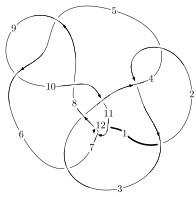
\includegraphics[width=112pt]{../../../GIT/diagram.site/Diagrams/png/2236_12n_0147.png}\\
\ \ \ A knot diagram\footnotemark}&
\allowdisplaybreaks
\textbf{Linearized knot diagam} \\
\cline{2-2}
 &
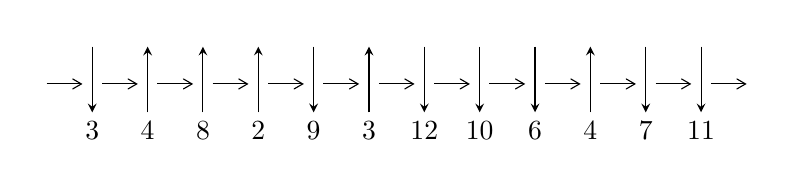
\begin{tikzpicture}[x=20pt, y=17pt]
	% nodes
	\node (C0) at (0, 0) {};
	\node (C1) at (1, 0) {};
	\node (C1U) at (1, +1) {};
	\node (C1D) at (1, -1) {3};

	\node (C2) at (2, 0) {};
	\node (C2U) at (2, +1) {};
	\node (C2D) at (2, -1) {4};

	\node (C3) at (3, 0) {};
	\node (C3U) at (3, +1) {};
	\node (C3D) at (3, -1) {8};

	\node (C4) at (4, 0) {};
	\node (C4U) at (4, +1) {};
	\node (C4D) at (4, -1) {2};

	\node (C5) at (5, 0) {};
	\node (C5U) at (5, +1) {};
	\node (C5D) at (5, -1) {9};

	\node (C6) at (6, 0) {};
	\node (C6U) at (6, +1) {};
	\node (C6D) at (6, -1) {3};

	\node (C7) at (7, 0) {};
	\node (C7U) at (7, +1) {};
	\node (C7D) at (7, -1) {12};

	\node (C8) at (8, 0) {};
	\node (C8U) at (8, +1) {};
	\node (C8D) at (8, -1) {10};

	\node (C9) at (9, 0) {};
	\node (C9U) at (9, +1) {};
	\node (C9D) at (9, -1) {6};

	\node (C10) at (10, 0) {};
	\node (C10U) at (10, +1) {};
	\node (C10D) at (10, -1) {4};

	\node (C11) at (11, 0) {};
	\node (C11U) at (11, +1) {};
	\node (C11D) at (11, -1) {7};

	\node (C12) at (12, 0) {};
	\node (C12U) at (12, +1) {};
	\node (C12D) at (12, -1) {11};
	\node (C13) at (13, 0) {};

	% arrows
	\draw[->,>={angle 60}]
	(C0) edge (C1) (C1) edge (C2) (C2) edge (C3) (C3) edge (C4) (C4) edge (C5) (C5) edge (C6) (C6) edge (C7) (C7) edge (C8) (C8) edge (C9) (C9) edge (C10) (C10) edge (C11) (C11) edge (C12) (C12) edge (C13) ;	\draw[->,>=stealth]
	(C1U) edge (C1D) (C2D) edge (C2U) (C3D) edge (C3U) (C4D) edge (C4U) (C5U) edge (C5D) (C6D) edge (C6U) (C7U) edge (C7D) (C8U) edge (C8D) (C9U) edge (C9D) (C10D) edge (C10U) (C11U) edge (C11D) (C12U) edge (C12D) ;
	\end{tikzpicture} \\
\hhline{~~} \\& 
\textbf{Solving Sequence} \\ \cline{2-2} 
 &
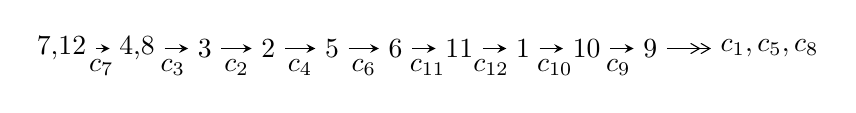
\begin{tikzpicture}[x=23pt, y=7pt]
	% node
	\node (A0) at (-1/8, 0) {7,12};
	\node (A1) at (17/16, 0) {4,8};
	\node (A2) at (17/8, 0) {3};
	\node (A3) at (25/8, 0) {2};
	\node (A4) at (33/8, 0) {5};
	\node (A5) at (41/8, 0) {6};
	\node (A6) at (49/8, 0) {11};
	\node (A7) at (57/8, 0) {1};
	\node (A8) at (65/8, 0) {10};
	\node (A9) at (73/8, 0) {9};
	\node (C1) at (1/2, -1) {$c_{7}$};
	\node (C2) at (13/8, -1) {$c_{3}$};
	\node (C3) at (21/8, -1) {$c_{2}$};
	\node (C4) at (29/8, -1) {$c_{4}$};
	\node (C5) at (37/8, -1) {$c_{6}$};
	\node (C6) at (45/8, -1) {$c_{11}$};
	\node (C7) at (53/8, -1) {$c_{12}$};
	\node (C8) at (61/8, -1) {$c_{10}$};
	\node (C9) at (69/8, -1) {$c_{9}$};
	\node (A10) at (11, 0) {$c_{1},c_{5},c_{8}$};

	% edge
	\draw[->,>=stealth]	
	(A0) edge (A1) (A1) edge (A2) (A2) edge (A3) (A3) edge (A4) (A4) edge (A5) (A5) edge (A6) (A6) edge (A7) (A7) edge (A8) (A8) edge (A9) ;
	\draw[->>,>={angle 60}]	
	(A9) edge (A10);
\end{tikzpicture} \\ 

\end{tabular} \\

\footnotetext{
The image of knot diagram is generated by the software ``\textbf{Draw programme}" developed by Andrew Bartholomew(\url{http://www.layer8.co.uk/maths/draw/index.htm\#Running-draw}), where we modified some parts for our purpose(\url{https://github.com/CATsTAILs/LinksPainter}).
}\phantom \\ \newline 
\centering \textbf{Ideals for irreducible components\footnotemark of $X_{\text{par}}$} 
 
\begin{align*}
I^u_{1}&=\langle 
-3 u^{15}-5 u^{14}+\cdots+4 b-5,\;-3 u^{15}-3 u^{14}+\cdots+2 a-4,\\
\phantom{I^u_{1}}&\phantom{= \langle  }u^{16}+u^{15}-5 u^{14}-5 u^{13}+11 u^{12}+12 u^{11}-8 u^{10}-13 u^9-8 u^8+2 u^7+18 u^6+11 u^5-7 u^4-9 u^3- u^2+2 u+1\rangle \\
I^u_{2}&=\langle 
1404675088 u^{27}+680434033 u^{26}+\cdots+5440114508 b+183536430,\\
\phantom{I^u_{2}}&\phantom{= \langle  }4259487893 u^{27}+5117778300 u^{26}+\cdots+10880229016 a-10842072870,\\
\phantom{I^u_{2}}&\phantom{= \langle  }u^{28}+2 u^{27}+\cdots+12 u+4\rangle \\
I^u_{3}&=\langle 
u^3+b+u+1,\;- u^2+a+2 u+1,\;u^4- u^2+1\rangle \\
I^u_{4}&=\langle 
- u^3+b- u+1,\;- u^2+a- u+1,\;u^4- u^2+1\rangle \\
I^u_{5}&=\langle 
- u^3+u^2+b- u-1,\;u^2+a- u,\;u^4- u^2+1\rangle \\
I^u_{6}&=\langle 
u^3- u^2+b+u,\;a+2 u-1,\;u^4- u^2+1\rangle \\
I^u_{7}&=\langle 
- u^3+b- u,\;a- u,\;u^4+u^3+1\rangle \\
I^u_{8}&=\langle 
a^3+2 a^2+b+3 a+1,\;a^4+3 a^3+6 a^2+4 a+1,\;u-1\rangle \\
I^u_{9}&=\langle 
b-2,\;a-1,\;u-1\rangle \\
\\
\end{align*}
\raggedright * 9 irreducible components of $\dim_{\mathbb{C}}=0$, with total 69 representations.\\
\footnotetext{All coefficients of polynomials are rational numbers. But the coefficients are sometimes approximated in decimal forms when there is not enough margin.}
\newpage
\renewcommand{\arraystretch}{1}
\centering \section*{I. $I^u_{1}= \langle -3 u^{15}-5 u^{14}+\cdots+4 b-5,\;-3 u^{15}-3 u^{14}+\cdots+2 a-4,\;u^{16}+u^{15}+\cdots+2 u+1 \rangle$}
\flushleft \textbf{(i) Arc colorings}\\
\begin{tabular}{m{7pt} m{180pt} m{7pt} m{180pt} }
\flushright $a_{7}=$&$\begin{pmatrix}1\\0\end{pmatrix}$ \\
\flushright $a_{12}=$&$\begin{pmatrix}0\\u\end{pmatrix}$ \\
\flushright $a_{4}=$&$\begin{pmatrix}\frac{3}{2} u^{15}+\frac{3}{2} u^{14}+\cdots+\frac{5}{2} u+2\\\frac{3}{4} u^{15}+\frac{5}{4} u^{14}+\cdots+\frac{1}{2} u+\frac{5}{4}\end{pmatrix}$ \\
\flushright $a_{8}=$&$\begin{pmatrix}1\\u^2\end{pmatrix}$ \\
\flushright $a_{3}=$&$\begin{pmatrix}\frac{1}{4} u^{15}+\frac{3}{4} u^{14}+\cdots+\frac{1}{2} u+\frac{3}{4}\\\frac{1}{2} u^{15}+\frac{3}{4} u^{14}+\cdots+\frac{3}{4} u+\frac{3}{4}\end{pmatrix}$ \\
\flushright $a_{2}=$&$\begin{pmatrix}-\frac{11}{4} u^{15}- u^{14}+\cdots-\frac{17}{4} u-\frac{7}{2}\\- u^{15}-\frac{1}{2} u^{14}+\cdots-\frac{1}{2} u-\frac{3}{2}\end{pmatrix}$ \\
\flushright $a_{5}=$&$\begin{pmatrix}\frac{5}{2} u^{15}+u^{14}+\cdots+\frac{9}{2} u+2\\u^{15}+\frac{1}{2} u^{14}+\cdots+\frac{3}{2} u+\frac{3}{2}\end{pmatrix}$ \\
\flushright $a_{6}=$&$\begin{pmatrix}-2 u^{15}-\frac{3}{4} u^{14}+\cdots-\frac{13}{4} u-\frac{5}{4}\\-\frac{3}{4} u^{15}-\frac{1}{4} u^{14}+\cdots-\frac{3}{2} u-\frac{5}{4}\end{pmatrix}$ \\
\flushright $a_{11}=$&$\begin{pmatrix}u\\u\end{pmatrix}$ \\
\flushright $a_{1}=$&$\begin{pmatrix}- u^3\\- u^3+u\end{pmatrix}$ \\
\flushright $a_{10}=$&$\begin{pmatrix}-2 u^{15}-\frac{3}{4} u^{14}+\cdots-\frac{13}{4} u-\frac{9}{4}\\-\frac{3}{4} u^{15}-\frac{1}{4} u^{14}+\cdots-\frac{1}{2} u-\frac{5}{4}\end{pmatrix}$ \\
\flushright $a_{9}=$&$\begin{pmatrix}-\frac{3}{4} u^{15}-\frac{1}{4} u^{14}+\cdots-\frac{1}{2} u-\frac{1}{4}\\-\frac{1}{4} u^{15}+\frac{3}{2} u^{13}+\cdots-\frac{1}{4} u-\frac{1}{2}\end{pmatrix}$\\&\end{tabular}
\flushleft \textbf{(ii) Obstruction class $= -1$}\\~\\
\flushleft \textbf{(iii) Cusp Shapes $= -6 u^{15}-\frac{1}{2} u^{14}+32 u^{13}+u^{12}-\frac{151}{2} u^{11}-4 u^{10}+\frac{147}{2} u^9+\frac{29}{2} u^8+\frac{21}{2} u^7-30 u^6-\frac{159}{2} u^5+\frac{41}{2} u^4+\frac{103}{2} u^3+\frac{5}{2} u^2-\frac{35}{2} u-\frac{13}{2}$}\\~\\
\newpage\renewcommand{\arraystretch}{1}
\flushleft \textbf{(iv) u-Polynomials at the component}\newline \\
\begin{tabular}{m{50pt}|m{274pt}}
Crossings & \hspace{64pt}u-Polynomials at each crossing \\
\hline $$\begin{aligned}c_{1}\end{aligned}$$&$\begin{aligned}
&u^{16}+16 u^{15}+\cdots+1760 u+256
\end{aligned}$\\
\hline $$\begin{aligned}c_{2},c_{4}\end{aligned}$$&$\begin{aligned}
&u^{16}-4 u^{15}+\cdots-56 u+16
\end{aligned}$\\
\hline $$\begin{aligned}c_{3}\end{aligned}$$&$\begin{aligned}
&u^{16}+4 u^{15}+\cdots+12 u+4
\end{aligned}$\\
\hline $$\begin{aligned}c_{5},c_{7},c_{9}\\c_{11}\end{aligned}$$&$\begin{aligned}
&u^{16}- u^{15}+\cdots-2 u+1
\end{aligned}$\\
\hline $$\begin{aligned}c_{6},c_{10}\end{aligned}$$&$\begin{aligned}
&u^{16}- u^{15}+\cdots+64 u+16
\end{aligned}$\\
\hline $$\begin{aligned}c_{8},c_{12}\end{aligned}$$&$\begin{aligned}
&u^{16}+11 u^{15}+\cdots+6 u+1
\end{aligned}$\\
\hline
\end{tabular}\\~\\
\newpage\renewcommand{\arraystretch}{1}
\flushleft \textbf{(v) Riley Polynomials at the component}\newline \\
\begin{tabular}{m{50pt}|m{274pt}}
Crossings & \hspace{64pt}Riley Polynomials at each crossing \\
\hline $$\begin{aligned}c_{1}\end{aligned}$$&$\begin{aligned}
&y^{16}-24 y^{15}+\cdots-508416 y+65536
\end{aligned}$\\
\hline $$\begin{aligned}c_{2},c_{4}\end{aligned}$$&$\begin{aligned}
&y^{16}+16 y^{15}+\cdots+1760 y+256
\end{aligned}$\\
\hline $$\begin{aligned}c_{3}\end{aligned}$$&$\begin{aligned}
&y^{16}-4 y^{15}+\cdots-56 y+16
\end{aligned}$\\
\hline $$\begin{aligned}c_{5},c_{7},c_{9}\\c_{11}\end{aligned}$$&$\begin{aligned}
&y^{16}-11 y^{15}+\cdots-6 y+1
\end{aligned}$\\
\hline $$\begin{aligned}c_{6},c_{10}\end{aligned}$$&$\begin{aligned}
&y^{16}+25 y^{15}+\cdots+256 y+256
\end{aligned}$\\
\hline $$\begin{aligned}c_{8},c_{12}\end{aligned}$$&$\begin{aligned}
&y^{16}-7 y^{15}+\cdots+10 y+1
\end{aligned}$\\
\hline
\end{tabular}\\~\\
\newpage\flushleft \textbf{(vi) Complex Volumes and Cusp Shapes}
$$\begin{array}{c|c|c}  
\text{Solutions to }I^u_{1}& \I (\text{vol} + \sqrt{-1}CS) & \text{Cusp shape}\\
 \hline 
\begin{aligned}
u &= -0.053870 + 0.977866 I \\
a &= \phantom{-}1.287840 - 0.220850 I \\
b &= -0.321900 - 0.803375 I\end{aligned}
 & -5.56822 - 3.25567 I & -1.25924 + 2.26983 I \\ \hline\begin{aligned}
u &= -0.053870 - 0.977866 I \\
a &= \phantom{-}1.287840 + 0.220850 I \\
b &= -0.321900 + 0.803375 I\end{aligned}
 & -5.56822 + 3.25567 I & -1.25924 - 2.26983 I \\ \hline\begin{aligned}
u &= \phantom{-}1.201500 + 0.360870 I \\
a &= -1.62412 - 1.03706 I \\
b &= -2.42883 - 2.34865 I\end{aligned}
 & -3.59239 - 7.60004 I & -5.70207 + 6.90528 I \\ \hline\begin{aligned}
u &= \phantom{-}1.201500 - 0.360870 I \\
a &= -1.62412 + 1.03706 I \\
b &= -2.42883 + 2.34865 I\end{aligned}
 & -3.59239 + 7.60004 I & -5.70207 - 6.90528 I \\ \hline\begin{aligned}
u &= -0.670764 + 0.317932 I \\
a &= \phantom{-}2.23583 - 1.40717 I \\
b &= \phantom{-}1.14025 - 0.90622 I\end{aligned}
 & -0.26009 + 4.34202 I & -3.06611 - 5.18312 I \\ \hline\begin{aligned}
u &= -0.670764 - 0.317932 I \\
a &= \phantom{-}2.23583 + 1.40717 I \\
b &= \phantom{-}1.14025 + 0.90622 I\end{aligned}
 & -0.26009 - 4.34202 I & -3.06611 + 5.18312 I \\ \hline\begin{aligned}
u &= \phantom{-}0.703515 + 0.140913 I \\
a &= \phantom{-}0.003040 + 0.299544 I \\
b &= \phantom{-}0.501025 + 0.546651 I\end{aligned}
 & -1.337230 - 0.185301 I & -7.62381 + 0.24647 I \\ \hline\begin{aligned}
u &= \phantom{-}0.703515 - 0.140913 I \\
a &= \phantom{-}0.003040 - 0.299544 I \\
b &= \phantom{-}0.501025 - 0.546651 I\end{aligned}
 & -1.337230 + 0.185301 I & -7.62381 - 0.24647 I \\ \hline\begin{aligned}
u &= -1.280950 + 0.212067 I \\
a &= \phantom{-}0.273114 - 0.087546 I \\
b &= \phantom{-}0.130376 + 0.667731 I\end{aligned}
 & -6.90379 + 2.57028 I & -9.79223 - 1.93561 I \\ \hline\begin{aligned}
u &= -1.280950 - 0.212067 I \\
a &= \phantom{-}0.273114 + 0.087546 I \\
b &= \phantom{-}0.130376 - 0.667731 I\end{aligned}
 & -6.90379 - 2.57028 I & -9.79223 + 1.93561 I\\
 \hline 
 \end{array}$$\newpage$$\begin{array}{c|c|c}  
\text{Solutions to }I^u_{1}& \I (\text{vol} + \sqrt{-1}CS) & \text{Cusp shape}\\
 \hline 
\begin{aligned}
u &= \phantom{-}1.29321 + 0.59629 I \\
a &= \phantom{-}1.59347 + 1.06533 I \\
b &= \phantom{-}1.53873 + 2.99555 I\end{aligned}
 & -12.8610 - 14.5081 I & -5.76542 + 7.91129 I \\ \hline\begin{aligned}
u &= \phantom{-}1.29321 - 0.59629 I \\
a &= \phantom{-}1.59347 - 1.06533 I \\
b &= \phantom{-}1.53873 - 2.99555 I\end{aligned}
 & -12.8610 + 14.5081 I & -5.76542 - 7.91129 I \\ \hline\begin{aligned}
u &= -0.358572 + 0.446053 I \\
a &= -2.09650 + 0.59301 I \\
b &= -0.541243 + 0.861918 I\end{aligned}
 & \phantom{-}1.55250 - 0.72268 I & \phantom{-}4.27343 + 0.90071 I \\ \hline\begin{aligned}
u &= -0.358572 - 0.446053 I \\
a &= -2.09650 - 0.59301 I \\
b &= -0.541243 - 0.861918 I\end{aligned}
 & \phantom{-}1.55250 + 0.72268 I & \phantom{-}4.27343 - 0.90071 I \\ \hline\begin{aligned}
u &= -1.33407 + 0.55318 I \\
a &= -0.172674 - 0.381772 I \\
b &= -0.018408 - 1.337270 I\end{aligned}
 & -13.7981 + 7.5953 I & -7.06455 - 3.46610 I \\ \hline\begin{aligned}
u &= -1.33407 - 0.55318 I \\
a &= -0.172674 + 0.381772 I \\
b &= -0.018408 + 1.337270 I\end{aligned}
 & -13.7981 - 7.5953 I & -7.06455 + 3.46610 I\\
 \hline 
 \end{array}$$\newpage\newpage\renewcommand{\arraystretch}{1}
\centering \section*{II. $I^u_{2}= \langle 1.40\times10^{9} u^{27}+6.80\times10^{8} u^{26}+\cdots+5.44\times10^{9} b+1.84\times10^{8},\;4.26\times10^{9} u^{27}+5.12\times10^{9} u^{26}+\cdots+1.09\times10^{10} a-1.08\times10^{10},\;u^{28}+2 u^{27}+\cdots+12 u+4 \rangle$}
\flushleft \textbf{(i) Arc colorings}\\
\begin{tabular}{m{7pt} m{180pt} m{7pt} m{180pt} }
\flushright $a_{7}=$&$\begin{pmatrix}1\\0\end{pmatrix}$ \\
\flushright $a_{12}=$&$\begin{pmatrix}0\\u\end{pmatrix}$ \\
\flushright $a_{4}=$&$\begin{pmatrix}-0.391489 u^{27}-0.470374 u^{26}+\cdots-3.81459 u+0.996493\\-0.258207 u^{27}-0.125077 u^{26}+\cdots-0.732283 u-0.0337376\end{pmatrix}$ \\
\flushright $a_{8}=$&$\begin{pmatrix}1\\u^2\end{pmatrix}$ \\
\flushright $a_{3}=$&$\begin{pmatrix}-0.413924 u^{27}-0.597145 u^{26}+\cdots-5.26760 u-0.220183\\-0.0582121 u^{27}-0.0675302 u^{26}+\cdots+0.340267 u+0.293866\end{pmatrix}$ \\
\flushright $a_{2}=$&$\begin{pmatrix}-0.477856 u^{27}-0.996708 u^{26}+\cdots-13.3082 u-4.41263\\-0.112376 u^{27}-0.407794 u^{26}+\cdots-2.58251 u-1.23931\end{pmatrix}$ \\
\flushright $a_{5}=$&$\begin{pmatrix}0.954572 u^{27}+1.16393 u^{26}+\cdots+13.8778 u+5.23994\\0.578242 u^{27}+0.838640 u^{26}+\cdots+6.12426 u+2.98085\end{pmatrix}$ \\
\flushright $a_{6}=$&$\begin{pmatrix}-0.553377 u^{27}-0.805395 u^{26}+\cdots-4.19380 u-0.220141\\-0.289887 u^{27}-0.549598 u^{26}+\cdots-2.44368 u-1.38590\end{pmatrix}$ \\
\flushright $a_{11}=$&$\begin{pmatrix}u\\u\end{pmatrix}$ \\
\flushright $a_{1}=$&$\begin{pmatrix}- u^3\\- u^3+u\end{pmatrix}$ \\
\flushright $a_{10}=$&$\begin{pmatrix}-0.344773 u^{27}-0.559849 u^{26}+\cdots-12.5913 u-2.43833\\-0.107385 u^{27}-0.0325593 u^{26}+\cdots-1.42978 u-0.191489\end{pmatrix}$ \\
\flushright $a_{9}=$&$\begin{pmatrix}0.122884 u^{27}+0.0337522 u^{26}+\cdots-7.99636 u-2.60537\\-0.0118276 u^{27}+0.0954702 u^{26}+\cdots-1.56095 u-0.292717\end{pmatrix}$\\&\end{tabular}
\flushleft \textbf{(ii) Obstruction class $= -1$}\\~\\
\flushleft \textbf{(iii) Cusp Shapes $= -\frac{3864981188}{1360028627} u^{27}-\frac{4406004267}{1360028627} u^{26}+\cdots-\frac{49326955058}{1360028627} u-\frac{19445189018}{1360028627}$}\\~\\
\newpage\renewcommand{\arraystretch}{1}
\flushleft \textbf{(iv) u-Polynomials at the component}\newline \\
\begin{tabular}{m{50pt}|m{274pt}}
Crossings & \hspace{64pt}u-Polynomials at each crossing \\
\hline $$\begin{aligned}c_{1}\end{aligned}$$&$\begin{aligned}
&(u^{14}+21 u^{13}+\cdots-66 u+1)^{2}
\end{aligned}$\\
\hline $$\begin{aligned}c_{2},c_{4}\end{aligned}$$&$\begin{aligned}
&(u^{14}-3 u^{13}+\cdots-14 u+1)^{2}
\end{aligned}$\\
\hline $$\begin{aligned}c_{3}\end{aligned}$$&$\begin{aligned}
&(u^{14}- u^{13}+\cdots-2 u+1)^{2}
\end{aligned}$\\
\hline $$\begin{aligned}c_{5},c_{7},c_{9}\\c_{11}\end{aligned}$$&$\begin{aligned}
&u^{28}-2 u^{27}+\cdots-12 u+4
\end{aligned}$\\
\hline $$\begin{aligned}c_{6},c_{10}\end{aligned}$$&$\begin{aligned}
&u^{28}+5 u^{27}+\cdots+251482 u+48331
\end{aligned}$\\
\hline $$\begin{aligned}c_{8},c_{12}\end{aligned}$$&$\begin{aligned}
&u^{28}+16 u^{27}+\cdots-104 u+16
\end{aligned}$\\
\hline
\end{tabular}\\~\\
\newpage\renewcommand{\arraystretch}{1}
\flushleft \textbf{(v) Riley Polynomials at the component}\newline \\
\begin{tabular}{m{50pt}|m{274pt}}
Crossings & \hspace{64pt}Riley Polynomials at each crossing \\
\hline $$\begin{aligned}c_{1}\end{aligned}$$&$\begin{aligned}
&(y^{14}-59 y^{13}+\cdots-3858 y+1)^{2}
\end{aligned}$\\
\hline $$\begin{aligned}c_{2},c_{4}\end{aligned}$$&$\begin{aligned}
&(y^{14}+21 y^{13}+\cdots-66 y+1)^{2}
\end{aligned}$\\
\hline $$\begin{aligned}c_{3}\end{aligned}$$&$\begin{aligned}
&(y^{14}-3 y^{13}+\cdots-14 y+1)^{2}
\end{aligned}$\\
\hline $$\begin{aligned}c_{5},c_{7},c_{9}\\c_{11}\end{aligned}$$&$\begin{aligned}
&y^{28}-16 y^{27}+\cdots+104 y+16
\end{aligned}$\\
\hline $$\begin{aligned}c_{6},c_{10}\end{aligned}$$&$\begin{aligned}
&y^{28}+29 y^{27}+\cdots+1236737368 y+2335885561
\end{aligned}$\\
\hline $$\begin{aligned}c_{8},c_{12}\end{aligned}$$&$\begin{aligned}
&y^{28}-8 y^{27}+\cdots-14112 y+256
\end{aligned}$\\
\hline
\end{tabular}\\~\\
\newpage\flushleft \textbf{(vi) Complex Volumes and Cusp Shapes}
$$\begin{array}{c|c|c}  
\text{Solutions to }I^u_{2}& \I (\text{vol} + \sqrt{-1}CS) & \text{Cusp shape}\\
 \hline 
\begin{aligned}
u &= -0.944960 + 0.389379 I \\
a &= \phantom{-}1.68750 - 1.23439 I \\
b &= \phantom{-}1.31224 - 1.71461 I\end{aligned}
 & -0.06814 + 4.27159 I & -1.66019 - 6.67920 I \\ \hline\begin{aligned}
u &= -0.944960 - 0.389379 I \\
a &= \phantom{-}1.68750 + 1.23439 I \\
b &= \phantom{-}1.31224 + 1.71461 I\end{aligned}
 & -0.06814 - 4.27159 I & -1.66019 + 6.67920 I \\ \hline\begin{aligned}
u &= \phantom{-}0.167349 + 1.046550 I \\
a &= -1.56673 - 0.27072 I \\
b &= \phantom{-}0.750716 - 1.143810 I\end{aligned}
 & -9.38462 + 8.62895 I & -3.88181 - 4.95064 I \\ \hline\begin{aligned}
u &= \phantom{-}0.167349 - 1.046550 I \\
a &= -1.56673 + 0.27072 I \\
b &= \phantom{-}0.750716 + 1.143810 I\end{aligned}
 & -9.38462 - 8.62895 I & -3.88181 + 4.95064 I \\ \hline\begin{aligned}
u &= -0.071840 + 1.060620 I \\
a &= -1.156110 - 0.491907 I \\
b &= \phantom{-}0.349038 - 0.236829 I\end{aligned}
 & -9.86399 - 1.83809 I & -4.68358 + 0.51446 I \\ \hline\begin{aligned}
u &= -0.071840 - 1.060620 I \\
a &= -1.156110 + 0.491907 I \\
b &= \phantom{-}0.349038 + 0.236829 I\end{aligned}
 & -9.86399 + 1.83809 I & -4.68358 - 0.51446 I \\ \hline\begin{aligned}
u &= \phantom{-}0.930250 + 0.540185 I \\
a &= -0.39656 - 1.39984 I \\
b &= \phantom{-}0.82318 - 1.20145 I\end{aligned}
 & \phantom{-}0.178509\phantom{ +0.000000I} & -1.66494 + 0. I\phantom{ +0.000000I} \\ \hline\begin{aligned}
u &= \phantom{-}0.930250 - 0.540185 I \\
a &= -0.39656 + 1.39984 I \\
b &= \phantom{-}0.82318 + 1.20145 I\end{aligned}
 & \phantom{-}0.178509\phantom{ +0.000000I} & -1.66494 + 0. I\phantom{ +0.000000I} \\ \hline\begin{aligned}
u &= -0.967293 + 0.545264 I \\
a &= \phantom{-}1.19253 - 1.46190 I \\
b &= -0.09011 - 2.03761 I\end{aligned}
 & \phantom{-}0.97692 + 4.37418 I & \phantom{-}1.48632 - 5.65859 I \\ \hline\begin{aligned}
u &= -0.967293 - 0.545264 I \\
a &= \phantom{-}1.19253 + 1.46190 I \\
b &= -0.09011 + 2.03761 I\end{aligned}
 & \phantom{-}0.97692 - 4.37418 I & \phantom{-}1.48632 + 5.65859 I\\
 \hline 
 \end{array}$$\newpage$$\begin{array}{c|c|c}  
\text{Solutions to }I^u_{2}& \I (\text{vol} + \sqrt{-1}CS) & \text{Cusp shape}\\
 \hline 
\begin{aligned}
u &= -1.120270 + 0.185451 I \\
a &= \phantom{-}0.336290 + 0.781567 I \\
b &= \phantom{-}0.0603554 + 0.0344181 I\end{aligned}
 & -2.83422 + 5.28701 I & -7.29071 - 5.64998 I \\ \hline\begin{aligned}
u &= -1.120270 - 0.185451 I \\
a &= \phantom{-}0.336290 - 0.781567 I \\
b &= \phantom{-}0.0603554 - 0.0344181 I\end{aligned}
 & -2.83422 - 5.28701 I & -7.29071 + 5.64998 I \\ \hline\begin{aligned}
u &= \phantom{-}0.661296 + 0.516335 I \\
a &= \phantom{-}1.39638 - 1.24212 I \\
b &= \phantom{-}1.77737 + 0.58800 I\end{aligned}
 & \phantom{-}0.97692 - 4.37418 I & \phantom{-}1.48632 + 5.65859 I \\ \hline\begin{aligned}
u &= \phantom{-}0.661296 - 0.516335 I \\
a &= \phantom{-}1.39638 + 1.24212 I \\
b &= \phantom{-}1.77737 - 0.58800 I\end{aligned}
 & \phantom{-}0.97692 + 4.37418 I & \phantom{-}1.48632 - 5.65859 I \\ \hline\begin{aligned}
u &= \phantom{-}0.986837 + 0.702176 I \\
a &= -1.43243 - 0.29298 I \\
b &= -0.95756 - 1.34618 I\end{aligned}
 & -2.83422 - 5.28701 I & -7.29071 + 5.64998 I \\ \hline\begin{aligned}
u &= \phantom{-}0.986837 - 0.702176 I \\
a &= -1.43243 + 0.29298 I \\
b &= -0.95756 + 1.34618 I\end{aligned}
 & -2.83422 + 5.28701 I & -7.29071 - 5.64998 I \\ \hline\begin{aligned}
u &= -0.576536 + 0.519983 I \\
a &= -1.80604 - 0.49276 I \\
b &= -1.20129 + 1.05231 I\end{aligned}
 & \phantom{-}2.08354\phantom{ +0.000000I} & \phantom{-}4.91356 + 0. I\phantom{ +0.000000I} \\ \hline\begin{aligned}
u &= -0.576536 - 0.519983 I \\
a &= -1.80604 + 0.49276 I \\
b &= -1.20129 - 1.05231 I\end{aligned}
 & \phantom{-}2.08354\phantom{ +0.000000I} & \phantom{-}4.91356 + 0. I\phantom{ +0.000000I} \\ \hline\begin{aligned}
u &= -1.296330 + 0.525251 I \\
a &= -1.29110 + 1.10158 I \\
b &= -1.32954 + 2.42151 I\end{aligned}
 & -9.38462 + 8.62895 I & -3.88181 - 4.95064 I \\ \hline\begin{aligned}
u &= -1.296330 - 0.525251 I \\
a &= -1.29110 - 1.10158 I \\
b &= -1.32954 - 2.42151 I\end{aligned}
 & -9.38462 - 8.62895 I & -3.88181 + 4.95064 I\\
 \hline 
 \end{array}$$\newpage$$\begin{array}{c|c|c}  
\text{Solutions to }I^u_{2}& \I (\text{vol} + \sqrt{-1}CS) & \text{Cusp shape}\\
 \hline 
\begin{aligned}
u &= \phantom{-}1.323650 + 0.464051 I \\
a &= \phantom{-}0.131487 - 0.110768 I \\
b &= -0.532418 - 0.972507 I\end{aligned}
 & -9.86399 - 1.83809 I & -4.68358 + 0.51446 I \\ \hline\begin{aligned}
u &= \phantom{-}1.323650 - 0.464051 I \\
a &= \phantom{-}0.131487 + 0.110768 I \\
b &= -0.532418 + 0.972507 I\end{aligned}
 & -9.86399 + 1.83809 I & -4.68358 - 0.51446 I \\ \hline\begin{aligned}
u &= -1.39944 + 0.38754 I \\
a &= \phantom{-}0.184103 - 0.013266 I \\
b &= \phantom{-}1.29482 - 1.20212 I\end{aligned}
 & -14.5006 - 3.5759 I & -7.59435 + 2.22005 I \\ \hline\begin{aligned}
u &= -1.39944 - 0.38754 I \\
a &= \phantom{-}0.184103 + 0.013266 I \\
b &= \phantom{-}1.29482 + 1.20212 I\end{aligned}
 & -14.5006 + 3.5759 I & -7.59435 - 2.22005 I \\ \hline\begin{aligned}
u &= \phantom{-}1.38126 + 0.46460 I \\
a &= \phantom{-}1.074130 + 0.763312 I \\
b &= \phantom{-}1.81408 + 1.69170 I\end{aligned}
 & -14.5006 - 3.5759 I & -7.59435 + 2.22005 I \\ \hline\begin{aligned}
u &= \phantom{-}1.38126 - 0.46460 I \\
a &= \phantom{-}1.074130 - 0.763312 I \\
b &= \phantom{-}1.81408 - 1.69170 I\end{aligned}
 & -14.5006 + 3.5759 I & -7.59435 - 2.22005 I \\ \hline\begin{aligned}
u &= -0.073973 + 0.383908 I \\
a &= \phantom{-}3.89655 + 0.21962 I \\
b &= \phantom{-}0.429118 + 0.189827 I\end{aligned}
 & -0.06814 + 4.27159 I & -1.66019 - 6.67920 I \\ \hline\begin{aligned}
u &= -0.073973 - 0.383908 I \\
a &= \phantom{-}3.89655 - 0.21962 I \\
b &= \phantom{-}0.429118 - 0.189827 I\end{aligned}
 & -0.06814 - 4.27159 I & -1.66019 + 6.67920 I\\
 \hline 
 \end{array}$$\newpage\newpage\renewcommand{\arraystretch}{1}
\centering \section*{III. $I^u_{3}= \langle u^3+b+u+1,\;- u^2+a+2 u+1,\;u^4- u^2+1 \rangle$}
\flushleft \textbf{(i) Arc colorings}\\
\begin{tabular}{m{7pt} m{180pt} m{7pt} m{180pt} }
\flushright $a_{7}=$&$\begin{pmatrix}1\\0\end{pmatrix}$ \\
\flushright $a_{12}=$&$\begin{pmatrix}0\\u\end{pmatrix}$ \\
\flushright $a_{4}=$&$\begin{pmatrix}u^2-2 u-1\\- u^3- u-1\end{pmatrix}$ \\
\flushright $a_{8}=$&$\begin{pmatrix}1\\u^2\end{pmatrix}$ \\
\flushright $a_{3}=$&$\begin{pmatrix}- u^3+u^2- u-1\\- u^3-1\end{pmatrix}$ \\
\flushright $a_{2}=$&$\begin{pmatrix}-3 u^3+u-1\\-2 u^3- u^2+2 u\end{pmatrix}$ \\
\flushright $a_{5}=$&$\begin{pmatrix}u^3\\u^3- u\end{pmatrix}$ \\
\flushright $a_{6}=$&$\begin{pmatrix}u^3+2 u\\2 u^3\end{pmatrix}$ \\
\flushright $a_{11}=$&$\begin{pmatrix}u\\u\end{pmatrix}$ \\
\flushright $a_{1}=$&$\begin{pmatrix}- u^3\\- u^3+u\end{pmatrix}$ \\
\flushright $a_{10}=$&$\begin{pmatrix}3 u^2-3\\u^2-3\end{pmatrix}$ \\
\flushright $a_{9}=$&$\begin{pmatrix}-2\\- u^2-1\end{pmatrix}$\\&\end{tabular}
\flushleft \textbf{(ii) Obstruction class $= 1$}\\~\\
\flushleft \textbf{(iii) Cusp Shapes $= 12 u^2-8$}\\~\\
\newpage\renewcommand{\arraystretch}{1}
\flushleft \textbf{(iv) u-Polynomials at the component}\newline \\
\begin{tabular}{m{50pt}|m{274pt}}
Crossings & \hspace{64pt}u-Polynomials at each crossing \\
\hline $$\begin{aligned}c_{1},c_{4},c_{8}\end{aligned}$$&$\begin{aligned}
&(u^2- u+1)^2
\end{aligned}$\\
\hline $$\begin{aligned}c_{2},c_{12}\end{aligned}$$&$\begin{aligned}
&(u^2+u+1)^2
\end{aligned}$\\
\hline $$\begin{aligned}c_{3},c_{5},c_{7}\\c_{9},c_{11}\end{aligned}$$&$\begin{aligned}
&u^4- u^2+1
\end{aligned}$\\
\hline $$\begin{aligned}c_{6}\end{aligned}$$&$\begin{aligned}
&(u^2+2 u+2)^2
\end{aligned}$\\
\hline $$\begin{aligned}c_{10}\end{aligned}$$&$\begin{aligned}
&(u^2-2 u+2)^2
\end{aligned}$\\
\hline
\end{tabular}\\~\\
\newpage\renewcommand{\arraystretch}{1}
\flushleft \textbf{(v) Riley Polynomials at the component}\newline \\
\begin{tabular}{m{50pt}|m{274pt}}
Crossings & \hspace{64pt}Riley Polynomials at each crossing \\
\hline $$\begin{aligned}c_{1},c_{2},c_{4}\\c_{8},c_{12}\end{aligned}$$&$\begin{aligned}
&(y^2+y+1)^2
\end{aligned}$\\
\hline $$\begin{aligned}c_{3},c_{5},c_{7}\\c_{9},c_{11}\end{aligned}$$&$\begin{aligned}
&(y^2- y+1)^2
\end{aligned}$\\
\hline $$\begin{aligned}c_{6},c_{10}\end{aligned}$$&$\begin{aligned}
&(y^2+4)^2
\end{aligned}$\\
\hline
\end{tabular}\\~\\
\newpage\flushleft \textbf{(vi) Complex Volumes and Cusp Shapes}
$$\begin{array}{c|c|c}  
\text{Solutions to }I^u_{3}& \I (\text{vol} + \sqrt{-1}CS) & \text{Cusp shape}\\
 \hline 
\begin{aligned}
u &= \phantom{-}0.866025 + 0.500000 I \\
a &= -2.23205 - 0.13397 I \\
b &= -1.86603 - 1.50000 I\end{aligned}
 & \phantom{-0.000000 } -6.08965 I & -2.00000 + 10.39230 I \\ \hline\begin{aligned}
u &= \phantom{-}0.866025 - 0.500000 I \\
a &= -2.23205 + 0.13397 I \\
b &= -1.86603 + 1.50000 I\end{aligned}
 & \phantom{-0.000000 -}6.08965 I & -2.00000 - 10.39230 I \\ \hline\begin{aligned}
u &= -0.866025 + 0.500000 I \\
a &= \phantom{-}1.23205 - 1.86603 I \\
b &= -0.13397 - 1.50000 I\end{aligned}
 & \phantom{-0.000000 -}6.08965 I & -2.00000 - 10.39230 I \\ \hline\begin{aligned}
u &= -0.866025 - 0.500000 I \\
a &= \phantom{-}1.23205 + 1.86603 I \\
b &= -0.13397 + 1.50000 I\end{aligned}
 & \phantom{-0.000000 } -6.08965 I & -2.00000 + 10.39230 I\\
 \hline 
 \end{array}$$\newpage\newpage\renewcommand{\arraystretch}{1}
\centering \section*{IV. $I^u_{4}= \langle - u^3+b- u+1,\;- u^2+a- u+1,\;u^4- u^2+1 \rangle$}
\flushleft \textbf{(i) Arc colorings}\\
\begin{tabular}{m{7pt} m{180pt} m{7pt} m{180pt} }
\flushright $a_{7}=$&$\begin{pmatrix}1\\0\end{pmatrix}$ \\
\flushright $a_{12}=$&$\begin{pmatrix}0\\u\end{pmatrix}$ \\
\flushright $a_{4}=$&$\begin{pmatrix}u^2+u-1\\u^3+u-1\end{pmatrix}$ \\
\flushright $a_{8}=$&$\begin{pmatrix}1\\u^2\end{pmatrix}$ \\
\flushright $a_{3}=$&$\begin{pmatrix}u^2-1\\u-1\end{pmatrix}$ \\
\flushright $a_{2}=$&$\begin{pmatrix}- u^3+u^2\\-2 u^3+u^2+2 u-1\end{pmatrix}$ \\
\flushright $a_{5}=$&$\begin{pmatrix}u^3\\u^3- u\end{pmatrix}$ \\
\flushright $a_{6}=$&$\begin{pmatrix}u^3- u^2- u+2\\u^2-2 u+1\end{pmatrix}$ \\
\flushright $a_{11}=$&$\begin{pmatrix}u\\u\end{pmatrix}$ \\
\flushright $a_{1}=$&$\begin{pmatrix}- u^3\\- u^3+u\end{pmatrix}$ \\
\flushright $a_{10}=$&$\begin{pmatrix}u^3-2 u^2+u+1\\2 u^3-2 u^2- u+3\end{pmatrix}$ \\
\flushright $a_{9}=$&$\begin{pmatrix}- u^3- u^2+2 u\\u^3-2 u^2+u+1\end{pmatrix}$\\&\end{tabular}
\flushleft \textbf{(ii) Obstruction class $= 1$}\\~\\
\flushleft \textbf{(iii) Cusp Shapes $= -4 u^2$}\\~\\
\newpage\renewcommand{\arraystretch}{1}
\flushleft \textbf{(iv) u-Polynomials at the component}\newline \\
\begin{tabular}{m{50pt}|m{274pt}}
Crossings & \hspace{64pt}u-Polynomials at each crossing \\
\hline $$\begin{aligned}c_{1},c_{4},c_{8}\end{aligned}$$&$\begin{aligned}
&(u^2- u+1)^2
\end{aligned}$\\
\hline $$\begin{aligned}c_{2},c_{12}\end{aligned}$$&$\begin{aligned}
&(u^2+u+1)^2
\end{aligned}$\\
\hline $$\begin{aligned}c_{3},c_{5},c_{7}\\c_{9},c_{11}\end{aligned}$$&$\begin{aligned}
&u^4- u^2+1
\end{aligned}$\\
\hline $$\begin{aligned}c_{6}\end{aligned}$$&$\begin{aligned}
&u^4+4 u^3+5 u^2+2 u+1
\end{aligned}$\\
\hline $$\begin{aligned}c_{10}\end{aligned}$$&$\begin{aligned}
&u^4+2 u^3+5 u^2+4 u+1
\end{aligned}$\\
\hline
\end{tabular}\\~\\
\newpage\renewcommand{\arraystretch}{1}
\flushleft \textbf{(v) Riley Polynomials at the component}\newline \\
\begin{tabular}{m{50pt}|m{274pt}}
Crossings & \hspace{64pt}Riley Polynomials at each crossing \\
\hline $$\begin{aligned}c_{1},c_{2},c_{4}\\c_{8},c_{12}\end{aligned}$$&$\begin{aligned}
&(y^2+y+1)^2
\end{aligned}$\\
\hline $$\begin{aligned}c_{3},c_{5},c_{7}\\c_{9},c_{11}\end{aligned}$$&$\begin{aligned}
&(y^2- y+1)^2
\end{aligned}$\\
\hline $$\begin{aligned}c_{6}\end{aligned}$$&$\begin{aligned}
&y^4-6 y^3+11 y^2+6 y+1
\end{aligned}$\\
\hline $$\begin{aligned}c_{10}\end{aligned}$$&$\begin{aligned}
&y^4+6 y^3+11 y^2-6 y+1
\end{aligned}$\\
\hline
\end{tabular}\\~\\
\newpage\flushleft \textbf{(vi) Complex Volumes and Cusp Shapes}
$$\begin{array}{c|c|c}  
\text{Solutions to }I^u_{4}& \I (\text{vol} + \sqrt{-1}CS) & \text{Cusp shape}\\
 \hline 
\begin{aligned}
u &= \phantom{-}0.866025 + 0.500000 I \\
a &= \phantom{-}0.36603 + 1.36603 I \\
b &= -0.13397 + 1.50000 I\end{aligned}
 & \phantom{-0.000000 -}2.02988 I & -2.00000 - 3.46410 I \\ \hline\begin{aligned}
u &= \phantom{-}0.866025 - 0.500000 I \\
a &= \phantom{-}0.36603 - 1.36603 I \\
b &= -0.13397 - 1.50000 I\end{aligned}
 & \phantom{-0.000000 } -2.02988 I & -2.00000 + 3.46410 I \\ \hline\begin{aligned}
u &= -0.866025 + 0.500000 I \\
a &= -1.36603 - 0.36603 I \\
b &= -1.86603 + 1.50000 I\end{aligned}
 & \phantom{-0.000000 } -2.02988 I & -2.00000 + 3.46410 I \\ \hline\begin{aligned}
u &= -0.866025 - 0.500000 I \\
a &= -1.36603 + 0.36603 I \\
b &= -1.86603 - 1.50000 I\end{aligned}
 & \phantom{-0.000000 -}2.02988 I & -2.00000 - 3.46410 I\\
 \hline 
 \end{array}$$\newpage\newpage\renewcommand{\arraystretch}{1}
\centering \section*{V. $I^u_{5}= \langle - u^3+u^2+b- u-1,\;u^2+a- u,\;u^4- u^2+1 \rangle$}
\flushleft \textbf{(i) Arc colorings}\\
\begin{tabular}{m{7pt} m{180pt} m{7pt} m{180pt} }
\flushright $a_{7}=$&$\begin{pmatrix}1\\0\end{pmatrix}$ \\
\flushright $a_{12}=$&$\begin{pmatrix}0\\u\end{pmatrix}$ \\
\flushright $a_{4}=$&$\begin{pmatrix}- u^2+u\\u^3- u^2+u+1\end{pmatrix}$ \\
\flushright $a_{8}=$&$\begin{pmatrix}1\\u^2\end{pmatrix}$ \\
\flushright $a_{3}=$&$\begin{pmatrix}- u^2\\- u^2+u+1\end{pmatrix}$ \\
\flushright $a_{2}=$&$\begin{pmatrix}- u^3-1\\-2 u^3- u^2+2 u\end{pmatrix}$ \\
\flushright $a_{5}=$&$\begin{pmatrix}u^3\\u^3- u\end{pmatrix}$ \\
\flushright $a_{6}=$&$\begin{pmatrix}- u^3\\-2 u^3+2 u\end{pmatrix}$ \\
\flushright $a_{11}=$&$\begin{pmatrix}u\\u\end{pmatrix}$ \\
\flushright $a_{1}=$&$\begin{pmatrix}- u^3\\- u^3+u\end{pmatrix}$ \\
\flushright $a_{10}=$&$\begin{pmatrix}u^2+1\\3 u^2-1\end{pmatrix}$ \\
\flushright $a_{9}=$&$\begin{pmatrix}2 u^2\\3 u^2-3\end{pmatrix}$\\&\end{tabular}
\flushleft \textbf{(ii) Obstruction class $= 1$}\\~\\
\flushleft \textbf{(iii) Cusp Shapes $= 4 u^2-4$}\\~\\
\newpage\renewcommand{\arraystretch}{1}
\flushleft \textbf{(iv) u-Polynomials at the component}\newline \\
\begin{tabular}{m{50pt}|m{274pt}}
Crossings & \hspace{64pt}u-Polynomials at each crossing \\
\hline $$\begin{aligned}c_{1},c_{4},c_{8}\end{aligned}$$&$\begin{aligned}
&(u^2- u+1)^2
\end{aligned}$\\
\hline $$\begin{aligned}c_{2},c_{12}\end{aligned}$$&$\begin{aligned}
&(u^2+u+1)^2
\end{aligned}$\\
\hline $$\begin{aligned}c_{3},c_{5},c_{7}\\c_{9},c_{11}\end{aligned}$$&$\begin{aligned}
&u^4- u^2+1
\end{aligned}$\\
\hline $$\begin{aligned}c_{6}\end{aligned}$$&$\begin{aligned}
&u^4-2 u^3+2 u^2-4 u+4
\end{aligned}$\\
\hline $$\begin{aligned}c_{10}\end{aligned}$$&$\begin{aligned}
&u^4+2 u^3+2 u^2+4 u+4
\end{aligned}$\\
\hline
\end{tabular}\\~\\
\newpage\renewcommand{\arraystretch}{1}
\flushleft \textbf{(v) Riley Polynomials at the component}\newline \\
\begin{tabular}{m{50pt}|m{274pt}}
Crossings & \hspace{64pt}Riley Polynomials at each crossing \\
\hline $$\begin{aligned}c_{1},c_{2},c_{4}\\c_{8},c_{12}\end{aligned}$$&$\begin{aligned}
&(y^2+y+1)^2
\end{aligned}$\\
\hline $$\begin{aligned}c_{3},c_{5},c_{7}\\c_{9},c_{11}\end{aligned}$$&$\begin{aligned}
&(y^2- y+1)^2
\end{aligned}$\\
\hline $$\begin{aligned}c_{6},c_{10}\end{aligned}$$&$\begin{aligned}
&y^4-4 y^2+16
\end{aligned}$\\
\hline
\end{tabular}\\~\\
\newpage\flushleft \textbf{(vi) Complex Volumes and Cusp Shapes}
$$\begin{array}{c|c|c}  
\text{Solutions to }I^u_{5}& \I (\text{vol} + \sqrt{-1}CS) & \text{Cusp shape}\\
 \hline 
\begin{aligned}
u &= \phantom{-}0.866025 + 0.500000 I \\
a &= \phantom{-}0.366025 - 0.366025 I \\
b &= \phantom{-}1.36603 + 0.63397 I\end{aligned}
 & \phantom{-0.000000 } -2.02988 I & -2.00000 + 3.46410 I \\ \hline\begin{aligned}
u &= \phantom{-}0.866025 - 0.500000 I \\
a &= \phantom{-}0.366025 + 0.366025 I \\
b &= \phantom{-}1.36603 - 0.63397 I\end{aligned}
 & \phantom{-0.000000 -}2.02988 I & -2.00000 - 3.46410 I \\ \hline\begin{aligned}
u &= -0.866025 + 0.500000 I \\
a &= -1.36603 + 1.36603 I \\
b &= -0.36603 + 2.36603 I\end{aligned}
 & \phantom{-0.000000 -}2.02988 I & -2.00000 - 3.46410 I \\ \hline\begin{aligned}
u &= -0.866025 - 0.500000 I \\
a &= -1.36603 - 1.36603 I \\
b &= -0.36603 - 2.36603 I\end{aligned}
 & \phantom{-0.000000 } -2.02988 I & -2.00000 + 3.46410 I\\
 \hline 
 \end{array}$$\newpage\newpage\renewcommand{\arraystretch}{1}
\centering \section*{VI. $I^u_{6}= \langle u^3- u^2+b+u,\;a+2 u-1,\;u^4- u^2+1 \rangle$}
\flushleft \textbf{(i) Arc colorings}\\
\begin{tabular}{m{7pt} m{180pt} m{7pt} m{180pt} }
\flushright $a_{7}=$&$\begin{pmatrix}1\\0\end{pmatrix}$ \\
\flushright $a_{12}=$&$\begin{pmatrix}0\\u\end{pmatrix}$ \\
\flushright $a_{4}=$&$\begin{pmatrix}-2 u+1\\- u^3+u^2- u\end{pmatrix}$ \\
\flushright $a_{8}=$&$\begin{pmatrix}1\\u^2\end{pmatrix}$ \\
\flushright $a_{3}=$&$\begin{pmatrix}- u^3- u+1\\- u^3+u^2\end{pmatrix}$ \\
\flushright $a_{2}=$&$\begin{pmatrix}-3 u^3+u^2+u\\-2 u^3+u^2+2 u-1\end{pmatrix}$ \\
\flushright $a_{5}=$&$\begin{pmatrix}u^3\\u^3- u\end{pmatrix}$ \\
\flushright $a_{6}=$&$\begin{pmatrix}-3 u^3+2 u^2+u-1\\-2 u^3+u^2+2 u-2\end{pmatrix}$ \\
\flushright $a_{11}=$&$\begin{pmatrix}u\\u\end{pmatrix}$ \\
\flushright $a_{1}=$&$\begin{pmatrix}- u^3\\- u^3+u\end{pmatrix}$ \\
\flushright $a_{10}=$&$\begin{pmatrix}u^3-2 u+3\\- u^3+2 u^2- u+1\end{pmatrix}$ \\
\flushright $a_{9}=$&$\begin{pmatrix}2 u^3-3 u^2- u+4\\u^3-2 u+3\end{pmatrix}$\\&\end{tabular}
\flushleft \textbf{(ii) Obstruction class $= 1$}\\~\\
\flushleft \textbf{(iii) Cusp Shapes $= 4 u^2-4$}\\~\\
\newpage\renewcommand{\arraystretch}{1}
\flushleft \textbf{(iv) u-Polynomials at the component}\newline \\
\begin{tabular}{m{50pt}|m{274pt}}
Crossings & \hspace{64pt}u-Polynomials at each crossing \\
\hline $$\begin{aligned}c_{1},c_{4},c_{8}\end{aligned}$$&$\begin{aligned}
&(u^2- u+1)^2
\end{aligned}$\\
\hline $$\begin{aligned}c_{2},c_{12}\end{aligned}$$&$\begin{aligned}
&(u^2+u+1)^2
\end{aligned}$\\
\hline $$\begin{aligned}c_{3},c_{5},c_{7}\\c_{9},c_{11}\end{aligned}$$&$\begin{aligned}
&u^4- u^2+1
\end{aligned}$\\
\hline $$\begin{aligned}c_{6}\end{aligned}$$&$\begin{aligned}
&u^4-2 u^3+5 u^2-4 u+1
\end{aligned}$\\
\hline $$\begin{aligned}c_{10}\end{aligned}$$&$\begin{aligned}
&u^4-4 u^3+5 u^2-2 u+1
\end{aligned}$\\
\hline
\end{tabular}\\~\\
\newpage\renewcommand{\arraystretch}{1}
\flushleft \textbf{(v) Riley Polynomials at the component}\newline \\
\begin{tabular}{m{50pt}|m{274pt}}
Crossings & \hspace{64pt}Riley Polynomials at each crossing \\
\hline $$\begin{aligned}c_{1},c_{2},c_{4}\\c_{8},c_{12}\end{aligned}$$&$\begin{aligned}
&(y^2+y+1)^2
\end{aligned}$\\
\hline $$\begin{aligned}c_{3},c_{5},c_{7}\\c_{9},c_{11}\end{aligned}$$&$\begin{aligned}
&(y^2- y+1)^2
\end{aligned}$\\
\hline $$\begin{aligned}c_{6}\end{aligned}$$&$\begin{aligned}
&y^4+6 y^3+11 y^2-6 y+1
\end{aligned}$\\
\hline $$\begin{aligned}c_{10}\end{aligned}$$&$\begin{aligned}
&y^4-6 y^3+11 y^2+6 y+1
\end{aligned}$\\
\hline
\end{tabular}\\~\\
\newpage\flushleft \textbf{(vi) Complex Volumes and Cusp Shapes}
$$\begin{array}{c|c|c}  
\text{Solutions to }I^u_{6}& \I (\text{vol} + \sqrt{-1}CS) & \text{Cusp shape}\\
 \hline 
\begin{aligned}
u &= \phantom{-}0.866025 + 0.500000 I \\
a &= -0.732051 - 1.000000 I \\
b &= -0.366025 - 0.633975 I\end{aligned}
 & \phantom{-0.000000 } -2.02988 I & -2.00000 + 3.46410 I \\ \hline\begin{aligned}
u &= \phantom{-}0.866025 - 0.500000 I \\
a &= -0.732051 + 1.000000 I \\
b &= -0.366025 + 0.633975 I\end{aligned}
 & \phantom{-0.000000 -}2.02988 I & -2.00000 - 3.46410 I \\ \hline\begin{aligned}
u &= -0.866025 + 0.500000 I \\
a &= \phantom{-}2.73205 - 1.00000 I \\
b &= \phantom{-}1.36603 - 2.36603 I\end{aligned}
 & \phantom{-0.000000 -}2.02988 I & -2.00000 - 3.46410 I \\ \hline\begin{aligned}
u &= -0.866025 - 0.500000 I \\
a &= \phantom{-}2.73205 + 1.00000 I \\
b &= \phantom{-}1.36603 + 2.36603 I\end{aligned}
 & \phantom{-0.000000 } -2.02988 I & -2.00000 + 3.46410 I\\
 \hline 
 \end{array}$$\newpage\newpage\renewcommand{\arraystretch}{1}
\centering \section*{VII. $I^u_{7}= \langle - u^3+b- u,\;a- u,\;u^4+u^3+1 \rangle$}
\flushleft \textbf{(i) Arc colorings}\\
\begin{tabular}{m{7pt} m{180pt} m{7pt} m{180pt} }
\flushright $a_{7}=$&$\begin{pmatrix}1\\0\end{pmatrix}$ \\
\flushright $a_{12}=$&$\begin{pmatrix}0\\u\end{pmatrix}$ \\
\flushright $a_{4}=$&$\begin{pmatrix}u\\u^3+u\end{pmatrix}$ \\
\flushright $a_{8}=$&$\begin{pmatrix}1\\u^2\end{pmatrix}$ \\
\flushright $a_{3}=$&$\begin{pmatrix}0\\u\end{pmatrix}$ \\
\flushright $a_{2}=$&$\begin{pmatrix}- u^3\\-2 u^3+2 u-1\end{pmatrix}$ \\
\flushright $a_{5}=$&$\begin{pmatrix}u^3+1\\u^3+u^2- u+2\end{pmatrix}$ \\
\flushright $a_{6}=$&$\begin{pmatrix}1\\u^2\end{pmatrix}$ \\
\flushright $a_{11}=$&$\begin{pmatrix}u\\u\end{pmatrix}$ \\
\flushright $a_{1}=$&$\begin{pmatrix}- u^3\\- u^3+u\end{pmatrix}$ \\
\flushright $a_{10}=$&$\begin{pmatrix}u^3+1\\u^3+u^2- u+2\end{pmatrix}$ \\
\flushright $a_{9}=$&$\begin{pmatrix}u^3+2\\u^3+2 u^2- u+2\end{pmatrix}$\\&\end{tabular}
\flushleft \textbf{(ii) Obstruction class $= -1$}\\~\\
\flushleft \textbf{(iii) Cusp Shapes $= -6$}\\~\\
\newpage\renewcommand{\arraystretch}{1}
\flushleft \textbf{(iv) u-Polynomials at the component}\newline \\
\begin{tabular}{m{50pt}|m{274pt}}
Crossings & \hspace{64pt}u-Polynomials at each crossing \\
\hline $$\begin{aligned}c_{1}\end{aligned}$$&$\begin{aligned}
&u^4+3 u^3+6 u^2+4 u+1
\end{aligned}$\\
\hline $$\begin{aligned}c_{2},c_{4}\end{aligned}$$&$\begin{aligned}
&u^4- u^3+2 u^2+1
\end{aligned}$\\
\hline $$\begin{aligned}c_{3},c_{6},c_{7}\\c_{11}\end{aligned}$$&$\begin{aligned}
&u^4- u^3+1
\end{aligned}$\\
\hline $$\begin{aligned}c_{5},c_{8},c_{9}\end{aligned}$$&$\begin{aligned}
&(u+1)^4
\end{aligned}$\\
\hline $$\begin{aligned}c_{10}\end{aligned}$$&$\begin{aligned}
&u^4-3 u^3+6 u^2-4 u+1
\end{aligned}$\\
\hline $$\begin{aligned}c_{12}\end{aligned}$$&$\begin{aligned}
&u^4+u^3+2 u^2+1
\end{aligned}$\\
\hline
\end{tabular}\\~\\
\newpage\renewcommand{\arraystretch}{1}
\flushleft \textbf{(v) Riley Polynomials at the component}\newline \\
\begin{tabular}{m{50pt}|m{274pt}}
Crossings & \hspace{64pt}Riley Polynomials at each crossing \\
\hline $$\begin{aligned}c_{1},c_{10}\end{aligned}$$&$\begin{aligned}
&y^4+3 y^3+14 y^2-4 y+1
\end{aligned}$\\
\hline $$\begin{aligned}c_{2},c_{4},c_{12}\end{aligned}$$&$\begin{aligned}
&y^4+3 y^3+6 y^2+4 y+1
\end{aligned}$\\
\hline $$\begin{aligned}c_{3},c_{6},c_{7}\\c_{11}\end{aligned}$$&$\begin{aligned}
&y^4- y^3+2 y^2+1
\end{aligned}$\\
\hline $$\begin{aligned}c_{5},c_{8},c_{9}\end{aligned}$$&$\begin{aligned}
&(y-1)^4
\end{aligned}$\\
\hline
\end{tabular}\\~\\
\newpage\flushleft \textbf{(vi) Complex Volumes and Cusp Shapes}
$$\begin{array}{c|c|c}  
\text{Solutions to }I^u_{7}& \I (\text{vol} + \sqrt{-1}CS) & \text{Cusp shape}\\
 \hline 
\begin{aligned}
u &= \phantom{-}0.518913 + 0.666610 I \\
a &= \phantom{-}0.518913 + 0.666610 I \\
b &= -0.033125 + 0.908884 I\end{aligned}
 & -1.64493\phantom{ +0.000000I} & -6.00000\phantom{ +0.000000I} \\ \hline\begin{aligned}
u &= \phantom{-}0.518913 - 0.666610 I \\
a &= \phantom{-}0.518913 - 0.666610 I \\
b &= -0.033125 - 0.908884 I\end{aligned}
 & -1.64493\phantom{ +0.000000I} & -6.00000\phantom{ +0.000000I} \\ \hline\begin{aligned}
u &= -1.018910 + 0.602565 I \\
a &= -1.018910 + 0.602565 I \\
b &= -0.96687 + 2.26050 I\end{aligned}
 & -1.64493\phantom{ +0.000000I} & -6.00000\phantom{ +0.000000I} \\ \hline\begin{aligned}
u &= -1.018910 - 0.602565 I \\
a &= -1.018910 - 0.602565 I \\
b &= -0.96687 - 2.26050 I\end{aligned}
 & -1.64493\phantom{ +0.000000I} & -6.00000\phantom{ +0.000000I}\\
 \hline 
 \end{array}$$\newpage\newpage\renewcommand{\arraystretch}{1}
\centering \section*{VIII. $I^u_{8}= \langle a^3+2 a^2+b+3 a+1,\;a^4+3 a^3+6 a^2+4 a+1,\;u-1 \rangle$}
\flushleft \textbf{(i) Arc colorings}\\
\begin{tabular}{m{7pt} m{180pt} m{7pt} m{180pt} }
\flushright $a_{7}=$&$\begin{pmatrix}1\\0\end{pmatrix}$ \\
\flushright $a_{12}=$&$\begin{pmatrix}0\\1\end{pmatrix}$ \\
\flushright $a_{4}=$&$\begin{pmatrix}a\\- a^3-2 a^2-3 a-1\end{pmatrix}$ \\
\flushright $a_{8}=$&$\begin{pmatrix}1\\1\end{pmatrix}$ \\
\flushright $a_{3}=$&$\begin{pmatrix}a^3+2 a^2+5 a+1\\a\end{pmatrix}$ \\
\flushright $a_{2}=$&$\begin{pmatrix}a^3+a^2+3 a\\- a^2\end{pmatrix}$ \\
\flushright $a_{5}=$&$\begin{pmatrix}-2 a-2\\-2 a-1\end{pmatrix}$ \\
\flushright $a_{6}=$&$\begin{pmatrix}- a^3- a^2-3 a\\a^2\end{pmatrix}$ \\
\flushright $a_{11}=$&$\begin{pmatrix}1\\1\end{pmatrix}$ \\
\flushright $a_{1}=$&$\begin{pmatrix}-1\\0\end{pmatrix}$ \\
\flushright $a_{10}=$&$\begin{pmatrix}a^3+2 a^2+3 a+2\\- a^2-2 a\end{pmatrix}$ \\
\flushright $a_{9}=$&$\begin{pmatrix}- a^3-4 a^2-6 a-1\\- a^3-4 a^2-5 a-1\end{pmatrix}$\\&\end{tabular}
\flushleft \textbf{(ii) Obstruction class $= -1$}\\~\\
\flushleft \textbf{(iii) Cusp Shapes $= -6$}\\~\\
\newpage\renewcommand{\arraystretch}{1}
\flushleft \textbf{(iv) u-Polynomials at the component}\newline \\
\begin{tabular}{m{50pt}|m{274pt}}
Crossings & \hspace{64pt}u-Polynomials at each crossing \\
\hline $$\begin{aligned}c_{1}\end{aligned}$$&$\begin{aligned}
&u^4+3 u^3+6 u^2+4 u+1
\end{aligned}$\\
\hline $$\begin{aligned}c_{2},c_{4}\end{aligned}$$&$\begin{aligned}
&u^4- u^3+2 u^2+1
\end{aligned}$\\
\hline $$\begin{aligned}c_{3},c_{5},c_{9}\\c_{10}\end{aligned}$$&$\begin{aligned}
&u^4- u^3+1
\end{aligned}$\\
\hline $$\begin{aligned}c_{6}\end{aligned}$$&$\begin{aligned}
&u^4-3 u^3+6 u^2-4 u+1
\end{aligned}$\\
\hline $$\begin{aligned}c_{7},c_{11},c_{12}\end{aligned}$$&$\begin{aligned}
&(u+1)^4
\end{aligned}$\\
\hline $$\begin{aligned}c_{8}\end{aligned}$$&$\begin{aligned}
&u^4+u^3+2 u^2+1
\end{aligned}$\\
\hline
\end{tabular}\\~\\
\newpage\renewcommand{\arraystretch}{1}
\flushleft \textbf{(v) Riley Polynomials at the component}\newline \\
\begin{tabular}{m{50pt}|m{274pt}}
Crossings & \hspace{64pt}Riley Polynomials at each crossing \\
\hline $$\begin{aligned}c_{1},c_{6}\end{aligned}$$&$\begin{aligned}
&y^4+3 y^3+14 y^2-4 y+1
\end{aligned}$\\
\hline $$\begin{aligned}c_{2},c_{4},c_{8}\end{aligned}$$&$\begin{aligned}
&y^4+3 y^3+6 y^2+4 y+1
\end{aligned}$\\
\hline $$\begin{aligned}c_{3},c_{5},c_{9}\\c_{10}\end{aligned}$$&$\begin{aligned}
&y^4- y^3+2 y^2+1
\end{aligned}$\\
\hline $$\begin{aligned}c_{7},c_{11},c_{12}\end{aligned}$$&$\begin{aligned}
&(y-1)^4
\end{aligned}$\\
\hline
\end{tabular}\\~\\
\newpage\flushleft \textbf{(vi) Complex Volumes and Cusp Shapes}
$$\begin{array}{c|c|c}  
\text{Solutions to }I^u_{8}& \I (\text{vol} + \sqrt{-1}CS) & \text{Cusp shape}\\
 \hline 
\begin{aligned}
u &= \phantom{-}1.00000\phantom{ +0.000000I} \\
a &= -0.447962 + 0.242275 I \\
b &= \phantom{-}0.070951 - 0.424335 I\end{aligned}
 & -1.64493\phantom{ +0.000000I} & -6.00000\phantom{ +0.000000I} \\ \hline\begin{aligned}
u &= \phantom{-}1.00000\phantom{ +0.000000I} \\
a &= -0.447962 - 0.242275 I \\
b &= \phantom{-}0.070951 + 0.424335 I\end{aligned}
 & -1.64493\phantom{ +0.000000I} & -6.00000\phantom{ +0.000000I} \\ \hline\begin{aligned}
u &= \phantom{-}1.00000\phantom{ +0.000000I} \\
a &= -1.05204 + 1.65794 I \\
b &= -2.07095 + 1.05537 I\end{aligned}
 & -1.64493\phantom{ +0.000000I} & -6.00000\phantom{ +0.000000I} \\ \hline\begin{aligned}
u &= \phantom{-}1.00000\phantom{ +0.000000I} \\
a &= -1.05204 - 1.65794 I \\
b &= -2.07095 - 1.05537 I\end{aligned}
 & -1.64493\phantom{ +0.000000I} & -6.00000\phantom{ +0.000000I}\\
 \hline 
 \end{array}$$\newpage\newpage\renewcommand{\arraystretch}{1}
\centering \section*{IX. $I^u_{9}= \langle b-2,\;a-1,\;u-1 \rangle$}
\flushleft \textbf{(i) Arc colorings}\\
\begin{tabular}{m{7pt} m{180pt} m{7pt} m{180pt} }
\flushright $a_{7}=$&$\begin{pmatrix}1\\0\end{pmatrix}$ \\
\flushright $a_{12}=$&$\begin{pmatrix}0\\1\end{pmatrix}$ \\
\flushright $a_{4}=$&$\begin{pmatrix}1\\2\end{pmatrix}$ \\
\flushright $a_{8}=$&$\begin{pmatrix}1\\1\end{pmatrix}$ \\
\flushright $a_{3}=$&$\begin{pmatrix}0\\1\end{pmatrix}$ \\
\flushright $a_{2}=$&$\begin{pmatrix}-1\\-1\end{pmatrix}$ \\
\flushright $a_{5}=$&$\begin{pmatrix}2\\3\end{pmatrix}$ \\
\flushright $a_{6}=$&$\begin{pmatrix}1\\1\end{pmatrix}$ \\
\flushright $a_{11}=$&$\begin{pmatrix}1\\1\end{pmatrix}$ \\
\flushright $a_{1}=$&$\begin{pmatrix}-1\\0\end{pmatrix}$ \\
\flushright $a_{10}=$&$\begin{pmatrix}2\\3\end{pmatrix}$ \\
\flushright $a_{9}=$&$\begin{pmatrix}3\\4\end{pmatrix}$\\&\end{tabular}
\flushleft \textbf{(ii) Obstruction class $= -1$}\\~\\
\flushleft \textbf{(iii) Cusp Shapes $= -6$}\\~\\
\newpage\renewcommand{\arraystretch}{1}
\flushleft \textbf{(iv) u-Polynomials at the component}\newline \\
\begin{tabular}{m{50pt}|m{274pt}}
Crossings & \hspace{64pt}u-Polynomials at each crossing \\
\hline $$\begin{aligned}c_{1},c_{2},c_{4}\end{aligned}$$&$\begin{aligned}
&u-1
\end{aligned}$\\
\hline $$\begin{aligned}c_{3},c_{5},c_{6}\\c_{7},c_{8},c_{9}\\c_{10},c_{11},c_{12}\end{aligned}$$&$\begin{aligned}
&u+1
\end{aligned}$\\
\hline
\end{tabular}\\~\\
\newpage\renewcommand{\arraystretch}{1}
\flushleft \textbf{(v) Riley Polynomials at the component}\newline \\
\begin{tabular}{m{50pt}|m{274pt}}
Crossings & \hspace{64pt}Riley Polynomials at each crossing \\
\hline $$\begin{aligned}c_{1},c_{2},c_{3}\\c_{4},c_{5},c_{6}\\c_{7},c_{8},c_{9}\\c_{10},c_{11},c_{12}\end{aligned}$$&$\begin{aligned}
&y-1
\end{aligned}$\\
\hline
\end{tabular}\\~\\
\newpage\flushleft \textbf{(vi) Complex Volumes and Cusp Shapes}
$$\begin{array}{c|c|c}  
\text{Solutions to }I^u_{9}& \I (\text{vol} + \sqrt{-1}CS) & \text{Cusp shape}\\
 \hline 
\begin{aligned}
u &= \phantom{-}1.00000\phantom{ +0.000000I} \\
a &= \phantom{-}1.00000\phantom{ +0.000000I} \\
b &= \phantom{-}2.00000\phantom{ +0.000000I}\end{aligned}
 & -1.64493\phantom{ +0.000000I} & -6.00000\phantom{ +0.000000I}\\
 \hline 
 \end{array}$$\newpage
\newpage\renewcommand{\arraystretch}{1}
\centering \section*{ X. u-Polynomials}
\begin{tabular}{m{50pt}|m{274pt}}
Crossings & \hspace{64pt}u-Polynomials at each crossing \\
\hline $$\begin{aligned}c_{1}\end{aligned}$$&$\begin{aligned}
&(u-1)(u^2- u+1)^8(u^4+3 u^3+6 u^2+4 u+1)^2\\
&\cdot((u^{14}+21 u^{13}+\cdots-66 u+1)^{2})(u^{16}+16 u^{15}+\cdots+1760 u+256)
\end{aligned}$\\
\hline $$\begin{aligned}c_{2}\end{aligned}$$&$\begin{aligned}
&(u-1)(u^2+u+1)^8(u^4- u^3+2 u^2+1)^{2}(u^{14}-3 u^{13}+\cdots-14 u+1)^{2}\\
&\cdot(u^{16}-4 u^{15}+\cdots-56 u+16)
\end{aligned}$\\
\hline $$\begin{aligned}c_{3}\end{aligned}$$&$\begin{aligned}
&(u+1)(u^4- u^2+1)^4(u^4- u^3+1)^2(u^{14}- u^{13}+\cdots-2 u+1)^{2}\\
&\cdot(u^{16}+4 u^{15}+\cdots+12 u+4)
\end{aligned}$\\
\hline $$\begin{aligned}c_{4}\end{aligned}$$&$\begin{aligned}
&(u-1)(u^2- u+1)^8(u^4- u^3+2 u^2+1)^{2}(u^{14}-3 u^{13}+\cdots-14 u+1)^{2}\\
&\cdot(u^{16}-4 u^{15}+\cdots-56 u+16)
\end{aligned}$\\
\hline $$\begin{aligned}c_{5},c_{7},c_{9}\\c_{11}\end{aligned}$$&$\begin{aligned}
&((u+1)^5)(u^4- u^2+1)^4(u^4- u^3+1)(u^{16}- u^{15}+\cdots-2 u+1)\\
&\cdot(u^{28}-2 u^{27}+\cdots-12 u+4)
\end{aligned}$\\
\hline $$\begin{aligned}c_{6}\end{aligned}$$&$\begin{aligned}
&(u+1)(u^2+2 u+2)^2(u^{4}-3 u^{3}+\cdots-4 u+1)(u^{4}-2 u^{3}+\cdots-4 u+4)\\
&\cdot(u^4-2 u^3+5 u^2-4 u+1)(u^4- u^3+1)(u^4+4 u^3+5 u^2+2 u+1)\\
&\cdot(u^{16}- u^{15}+\cdots+64 u+16)(u^{28}+5 u^{27}+\cdots+251482 u+48331)
\end{aligned}$\\
\hline $$\begin{aligned}c_{8}\end{aligned}$$&$\begin{aligned}
&((u+1)^5)(u^2- u+1)^8(u^4+u^3+2 u^2+1)(u^{16}+11 u^{15}+\cdots+6 u+1)\\
&\cdot(u^{28}+16 u^{27}+\cdots-104 u+16)
\end{aligned}$\\
\hline $$\begin{aligned}c_{10}\end{aligned}$$&$\begin{aligned}
&(u+1)(u^2-2 u+2)^2(u^{4}-4 u^{3}+\cdots-2 u+1)(u^{4}-3 u^{3}+\cdots-4 u+1)\\
&\cdot(u^4- u^3+1)(u^4+2 u^3+2 u^2+4 u+4)(u^4+2 u^3+5 u^2+4 u+1)\\
&\cdot(u^{16}- u^{15}+\cdots+64 u+16)(u^{28}+5 u^{27}+\cdots+251482 u+48331)
\end{aligned}$\\
\hline $$\begin{aligned}c_{12}\end{aligned}$$&$\begin{aligned}
&((u+1)^5)(u^2+u+1)^8(u^4+u^3+2 u^2+1)(u^{16}+11 u^{15}+\cdots+6 u+1)\\
&\cdot(u^{28}+16 u^{27}+\cdots-104 u+16)
\end{aligned}$\\
\hline
\end{tabular}\newpage\renewcommand{\arraystretch}{1}
\centering \section*{ XI. Riley Polynomials}
\begin{tabular}{m{50pt}|m{274pt}}
Crossings & \hspace{64pt}Riley Polynomials at each crossing \\
\hline $$\begin{aligned}c_{1}\end{aligned}$$&$\begin{aligned}
&(y-1)(y^2+y+1)^8(y^4+3 y^3+14 y^2-4 y+1)^2\\
&\cdot(y^{14}-59 y^{13}+\cdots-3858 y+1)^{2}\\
&\cdot(y^{16}-24 y^{15}+\cdots-508416 y+65536)
\end{aligned}$\\
\hline $$\begin{aligned}c_{2},c_{4}\end{aligned}$$&$\begin{aligned}
&(y-1)(y^2+y+1)^8(y^4+3 y^3+6 y^2+4 y+1)^2\\
&\cdot((y^{14}+21 y^{13}+\cdots-66 y+1)^{2})(y^{16}+16 y^{15}+\cdots+1760 y+256)
\end{aligned}$\\
\hline $$\begin{aligned}c_{3}\end{aligned}$$&$\begin{aligned}
&(y-1)(y^2- y+1)^8(y^4- y^3+2 y^2+1)^{2}(y^{14}-3 y^{13}+\cdots-14 y+1)^{2}\\
&\cdot(y^{16}-4 y^{15}+\cdots-56 y+16)
\end{aligned}$\\
\hline $$\begin{aligned}c_{5},c_{7},c_{9}\\c_{11}\end{aligned}$$&$\begin{aligned}
&((y-1)^5)(y^2- y+1)^8(y^4- y^3+2 y^2+1)(y^{16}-11 y^{15}+\cdots-6 y+1)\\
&\cdot(y^{28}-16 y^{27}+\cdots+104 y+16)
\end{aligned}$\\
\hline $$\begin{aligned}c_{6},c_{10}\end{aligned}$$&$\begin{aligned}
&(y-1)(y^2+4)^2(y^4-4 y^2+16)(y^4-6 y^3+11 y^2+6 y+1)\\
&\cdot(y^4- y^3+2 y^2+1)(y^4+3 y^3+\cdots-4 y+1)(y^4+6 y^3+\cdots-6 y+1)\\
&\cdot(y^{16}+25 y^{15}+\cdots+256 y+256)\\
&\cdot(y^{28}+29 y^{27}+\cdots+1236737368 y+2335885561)
\end{aligned}$\\
\hline $$\begin{aligned}c_{8},c_{12}\end{aligned}$$&$\begin{aligned}
&(y-1)^5(y^2+y+1)^8(y^4+3 y^3+6 y^2+4 y+1)\\
&\cdot(y^{16}-7 y^{15}+\cdots+10 y+1)(y^{28}-8 y^{27}+\cdots-14112 y+256)
\end{aligned}$\\
\hline
\end{tabular}
\vskip 2pc
\end{document}